%% Detecção Nativa em Nuvem de Ciberataques contra Estações Terrestres de Satélite
%%
%% Versão em português do manuscrito. Tradução de main.tex; os números, figuras
%% e tabelas vêm do mesmo paper/experiments.py, com vírgula decimal.
%%
%% Compilação:  make -C paper pt   (ou: latexmk -pdf main-pt.tex)
\documentclass[conference]{IEEEtran}
\IEEEoverridecommandlockouts

\usepackage[T1]{fontenc}
\usepackage[utf8]{inputenc}
\usepackage[brazil]{babel}
\usepackage{cite}
\usepackage{amsmath,amssymb}
\usepackage{graphicx}
\usepackage{booktabs}
\usepackage{multirow}
\usepackage{tikz}
\usepackage{xcolor}
\usepackage{url}
\usepackage[hidelinks,breaklinks]{hyperref}

\usetikzlibrary{arrows.meta,positioning,fit,backgrounds}

% Valores experimentais, gerados por paper/experiments.py.
\input{data/macros_pt}

\renewcommand{\abstractname}{Resumo}
\renewcommand{\IEEEkeywordsname}{Palavras-chave}

\definecolor{vizblue}{HTML}{2A78D6}
\definecolor{vizorange}{HTML}{EB6834}
\definecolor{vizaqua}{HTML}{1BAF7A}
\definecolor{vizink}{HTML}{52514E}

\begin{document}

\title{Detecção Nativa em Nuvem de Ciberataques\\
contra Estações Terrestres de Satélite:\\
Um Ambiente de Teste Aberto e Rotulado,\\ e Dois Resultados Negativos}

% A FAZER antes da submissão: substituir pelo nome completo e pela afiliação.
\author{\IEEEauthorblockN{Henrique}
\IEEEauthorblockA{\textit{Pesquisador independente}\\
\url{https://github.com/rikosoo/Cloud-Native-Detection-of-Cyberattacks-Against-Satellite-Ground-Stations}}}

\maketitle

\begin{abstract}
O segmento espacial de uma missão por satélite é caro de alcançar; o segmento
terrestre que o comanda é uma carga de trabalho de nuvem comum, com operadores,
credenciais, APIs e armazenamento de objetos. A pesquisa publicada em segurança
de satélites concentrou-se na espaçonave e no enlace de rádio, e não existe um
corpus aberto e rotulado contra o qual a detecção no segmento terrestre possa
ser medida. Apresentamos um ambiente de teste aberto que preenche essa lacuna:
uma estação terrestre simulada que emite quatro planos correlacionados de
evidência (telemetria da espaçonave, telecomandos autenticados, registros de
auditoria em nuvem e transferências de \emph{downlink}), cinco cenários de
emulação de adversário mapeados para SPARTA e MITRE ATT\&CK com verdade de
referência por evento, e uma pipeline de detecção nativa em nuvem com
\expRuleCount{} regras com estado mais uma linha de base de telemetria não
supervisionada, implantada na AWS por meio de Kinesis, Lambda, DynamoDB,
CloudTrail, GuardDuty e Security Hub. Ao longo de \expNumSeeds{} execuções
independentes de \expSimHours~horas, a pipeline detecta todos os cinco cenários
em todas as execuções, com precisão de $\expPrecision \pm \expPrecisionSD$ e
taxa de falsos positivos de \expFprOverall\% dos eventos benignos. A linha de
base aprendida é o que torna visível uma deriva comportamental sublimiar: ela
dispara $\expLeadMean \pm \expLeadSD$~minutos antes da primeira violação de
limite da espaçonave e eleva a revocação por evento daquele cenário de
\expRecAnomalyRules{} para \expRecAnomalousBehavior{}. Dois resultados
contrariam a justificativa de projeto da qual partimos. Primeiro, o modelo
multivariado não supera um detector por canal bem calibrado naquela deriva
($\mathrm{AUC}\ \expAucMulti \pm \expAucMultiSD$ contra
$\expAucUni \pm \expAucUniSD$). Segundo, uma sonda controlada que preserva todas
as distribuições marginais enquanto destrói a estrutura conjunta --- reproduzir
quadros de telemetria de meia órbita antes --- é invisível para ambos os
detectores ($\mathrm{AUC}\ \expAucSwapMulti$ e \expAucSwapUni{}, detectada em
\expSwapDetectedMulti{} de \expNumSeeds{} execuções), porque uma linha de base
ajustada sobre uma órbita inteira marginaliza exatamente a informação de fase que
o ataque viola. Encontramos também um limiar operacional abrupto: ajustar a linha
de base com menos de um ciclo diurno completo eleva a taxa de falsos positivos da
telemetria de \expFprFullDay\% para \expFprOneHour\%. Todo o código, os dados e
o arcabouço experimental são públicos.
\end{abstract}

\begin{IEEEkeywords}
estações terrestres de satélite, segurança de sistemas espaciais, detecção de
intrusão, detecção de anomalias, segurança em nuvem, emulação de adversário,
telemetria
\end{IEEEkeywords}

\section{Introdução}

Um satélite é difícil de atacar diretamente e difícil de reparar depois de
atacado. A estação terrestre que o comanda não é nem uma coisa nem outra.
Segmentos terrestres modernos são construídos com os mesmos componentes de
qualquer outra carga de trabalho em nuvem: provedores de identidade, endpoints
de API, filas de mensagens, armazenamento de objetos e os operadores que detêm
as credenciais. Um adversário que alcance o caminho de comando a partir daí
herda autoridade sobre o veículo sem nunca tocar em um rádio.

Trabalhos recentes tornaram o segmento espacial mensurável. Willbold et
al.~\cite{willbold2023space} realizaram a primeira análise sistemática de
segurança de software em \emph{firmware} real de satélites; Pavur et al.\
demonstraram interceptação em larga escala de enlaces operacionais de
satélite~\cite{pavur2020vsat} e defenderam uma agenda de pesquisa com artefatos
reproduzíveis~\cite{pavur2020sok}. A política seguiu o mesmo caminho, com a
\emph{Space Policy Directive-5} nomeando explicitamente o segmento terrestre
como parte do sistema protegido~\cite{spd5}, e a comunidade dispõe hoje de uma
taxonomia de adversários específica para o espaço no SPARTA~\cite{sparta}.

O que falta é aquilo que viabilizou o progresso na detecção de intrusão em
redes: um corpus aberto com verdade de referência. Levantamentos de conjuntos de
dados de IDS de rede listam dezenas de opções~\cite{ring2019datasets}; para o
segmento terrestre de satélites não existe, ao nosso conhecimento, nenhum.
Telemetria e registros de auditoria do segmento terrestre são
operacionalmente sensíveis e raramente publicados e, quando o são, vêm sem
rótulos. A consequência prática é que afirmações sobre detecção no segmento
terrestre não podem ser comparadas, e que o custo de um detector --- em falsos
positivos, em tempo de analista, em computação --- geralmente não é relatado.

Este artigo contribui com um ambiente de teste e uma avaliação, não com um novo
detector. Concretamente:

\begin{itemize}
  \item \textbf{Um gerador aberto e rotulado de corpus de estação terrestre}
  (Seção~\ref{sec:impl}). Uma estação simulada emite quatro planos
  correlacionados de evidência, e cinco cenários de emulação de adversário ---
  compromisso de credenciais, adulteração de telecomandos, reprodução
  (\emph{replay}), deriva comportamental sublimiar e exfiltração em massa ---
  injetam-se nessa linha temporal, rotulando todo evento que criam ou modificam.
  Os cenários se compõem: a sessão roubada estabelecida pelo estágio de
  credenciais é a mesma que os estágios de adulteração e exfiltração reutilizam.

  \item \textbf{Uma pipeline de detecção nativa em nuvem}
  (Seção~\ref{sec:design}). \expRuleCount{} regras com estado cobrindo
  identidade, integridade de comando, reprodução, limites da espaçonave e
  exfiltração, cada uma mapeada para uma técnica do ATT\&CK~\cite{attack} e
  emitida no \emph{AWS Security Finding Format}~\cite{asff}, mais uma linha de
  base de telemetria não supervisionada que executa dentro de uma função Lambda
  sem nenhum \emph{runtime} de aprendizado de máquina. O mesmo objeto de motor
  executa \emph{offline}, sob teste e na nuvem.

  \item \textbf{Uma avaliação medida, com resultados negativos}
  (Seções~\ref{sec:method}--\ref{sec:results}). Vinte execuções independentes,
  uma ablação separando as regras do modelo, uma comparação com as duas
  alternativas que uma missão real já possui (um detector por canal e as
  verificações de limite da própria espaçonave), uma sonda que isola a estrutura
  conjunta das marginais, uma varredura de sensibilidade ao tamanho da linha de
  base e o custo computacional. Dois dos achados contrariam a justificativa em
  torno da qual projetamos o modelo, e os relatamos como tais.
\end{itemize}

Organizamos a avaliação em torno de cinco perguntas:

\begin{description}
  \item[QP1] A pipeline detecta cada cenário, e com que precisão?
  \item[QP2] O que a linha de base aprendida acrescenta sobre as verificações de
  limite da própria espaçonave --- a alternativa que uma missão real já opera?
  \item[QP3] O modelo multivariado acrescenta algo sobre um detector por canal
  bem calibrado?
  \item[QP4] De quanta telemetria limpa a linha de base precisa antes de ser
  utilizável?
  \item[QP5] Quanto custa executar a pipeline?
\end{description}

\section{Contexto e Modelo de Ameaças}
\label{sec:background}

\subsection{O segmento terrestre como superfície de ataque}

Uma estação terrestre converte a intenção do operador em telecomandos
autenticados e o estado da espaçonave em produtos de dados arquivados. Quatro
tipos de registro são produzidos, e um detector precisa de todos os quatro:

\begin{enumerate}
  \item \emph{Telemetria.} Dados de bordo (\emph{housekeeping}) --- tensão e
  corrente do barramento, estado de carga da bateria, temperaturas do
  amplificador e da bateria, margem de enlace --- transmitidos continuamente
  durante um contato.
  \item \emph{Telecomandos.} Quadros TC do CCSDS~\cite{ccsds232}, autenticados em
  missões modernas pelo protocolo \emph{Space Data Link
  Security}~\cite{ccsds355}, que fornece uma etiqueta de autenticação com chave
  e um contador de sequência antirreprodução.
  \item \emph{Registros de auditoria em nuvem.} Atividade do plano de controle:
  quem entrou, de onde, com qual autenticador e quais APIs chamou.
  \item \emph{Transferências de \emph{downlink}.} Produtos de carga útil
  entrando (e potencialmente saindo) do arquivo da missão.
\end{enumerate}

Os dois primeiros descrevem o veículo; os dois últimos descrevem a empresa. A
maior parte da pesquisa publicada em segurança espacial trata dos dois
primeiros, e a maior parte das ferramentas corporativas de segurança trata dos
dois últimos. Uma intrusão atravessa de um lado a outro, e é essa observação que
fundamenta o projeto da Seção~\ref{sec:design}.

\subsection{Adversários}

Consideramos três perfis, seguindo as taxonomias
de~\cite{manulis2021newspace} e~\cite{falco2019principles}:

\emph{Oportunista.} \emph{Credential stuffing}, ferramentas de mercado, nenhum
conhecimento da missão. Alto volume, baixa furtividade. Interessado em
capacidade computacional e em extorquir o arquivo.

\emph{Interno.} Um operador credenciado agindo fora de seu papel. Usa
credenciais legítimas, de redes legítimas, em horários legítimos; apenas
\emph{o que} ele faz é anômalo. Derrota, por construção, toda regra baseada em
rede ou em procedência de identidade.

\emph{Patrocinado por Estado.} Paciente, conhecedor da missão, visa material
criptográfico e o caminho de comando, desativa o registro de auditoria
precocemente e prefere uma degradação indistinguível de uma falha de barramento
--- porque um operador que acredita que a espaçonave está com defeito agirá
segundo o procedimento errado.

\subsection{Fronteiras de confiança e caminhos de ataque}

Quatro fronteiras separam o operador do veículo: a fronteira humano-nuvem (B1,
defendida por autenticação multifator e política de rede), o plano de controle
da nuvem (B2, defendido por autorização de menor privilégio e registro de
auditoria), o \emph{uplink} (B3, defendido pela etiqueta de autenticação e pelo
contador de sequência) e a própria espaçonave (B4, defendida por verificações de
limite a bordo). A Tabela~\ref{tab:paths} lista os cinco caminhos de ataque que
emulamos, a fronteira que cada um atravessa e o mapeamento para
SPARTA~\cite{sparta} e ATT\&CK~\cite{attack}.

\begin{table*}[t]
\caption{Caminhos de ataque emulados, a fronteira de confiança que cada um atravessa e o mapeamento para os arcabouços.}
\label{tab:paths}
\centering
\footnotesize
\begin{tabular}{@{}llllp{0.35\textwidth}@{}}
\toprule
\textbf{Cenário} & \textbf{Fronteira} & \textbf{SPARTA} & \textbf{ATT\&CK} & \textbf{Ação do adversário} \\
\midrule
\texttt{credential\_compromise} & B1, B2 & IA-0004 & T1110.003, T1078.004, T1098.001 &
Pulverização de senhas, entrada sem MFA a partir de um bloco de rede não
confiável fora do horário de turno, nova chave de acesso, anexação de política
administrativa, trilha de auditoria apagada. \\
\texttt{command\_tampering} & B3 & EX-0012 & T1565.002 &
\emph{Opcode} e parâmetros reescritos em trânsito; uma etiqueta de autenticação
forjada com a chave errada; um comando fora do papel; uma inundação de
\emph{uplink}. \\
\texttt{replay} & B3 & EX-0013 & T1557 &
Quadros gravados retransmitidos literalmente horas depois. A etiqueta ainda
verifica: o adversário nunca deteve a chave~\cite{syverson1994replay}. \\
\texttt{anomalous\_behavior} & B4 & IMP-0002 & T1565.001 &
Degradação comandada em que cada canal permanece dentro de seus limites de
interface enquanto as relações entre eles se rompem. \\
\texttt{exfiltration} & B2 & EXF-0003 & T1530, T1537, T1567.002 &
Enumeração do arquivo, leituras em massa de objetos, cópia entre contas de
múltiplos gigabytes para um destino não aprovado. \\
\bottomrule
\end{tabular}
\end{table*}

\subsection{Pressupostos}

Assumimos que o fluxo de eventos chega ao detector: um adversário capaz de
suprimir telemetria silenciosamente derrota todas as regras, e é por isso que a
pipeline implantada alarma sobre a \emph{ausência} de eventos. Assumimos que o
registro de auditoria está ativo e tratamos sua desativação como, ela mesma, um
achado crítico. Assumimos que o material criptográfico dos telecomandos ainda
não foi roubado; quando é, a regra de integridade silencia e restam apenas as
regras comportamentais, razão pela qual o catálogo não se apoia somente na
etiqueta de autenticação.

\section{Projeto do Sistema}
\label{sec:design}

A Figura~\ref{fig:arch} mostra a pipeline. Três propriedades guiaram o projeto.

\emph{Um motor, três ambientes de execução.} O motor de detecção não importa
nenhum SDK de nuvem. Ele executa inalterado na ferramenta de linha de comando
\emph{offline}, na suíte de testes e dentro de uma função AWS Lambda. Os
serviços de nuvem são alcançados apenas por meio de uma interface de escoamento
de eventos e de uma interface de armazenamento de estado.

\emph{\emph{Offline} primeiro.} A pipeline completa --- gerar, ajustar,
detectar, pontuar --- executa com NumPy e um leitor de YAML, sem credenciais e
sem rede. É isso que torna o artefato reproduzível por um leitor que não tem
conta na AWS.

\emph{Medido, não afirmado.} Todo evento injetado carrega um rótulo de verdade
de referência, de modo que precisão, revocação e latência de detecção são
calculadas, não alegadas.

\begin{figure}[t]
\centering
\begin{tikzpicture}[
  x=1mm, y=1mm,
  font=\scriptsize,
  box/.style={draw=vizink!60, rounded corners=1pt, align=center,
              inner sep=1.2mm, minimum height=6mm, fill=white},
  src/.style={box, draw=vizblue, thick},
  det/.style={box, draw=vizorange, thick},
  sink/.style={box, draw=vizaqua, thick},
  arr/.style={-{Stealth[length=1.3mm]}, draw=vizink, line width=0.4pt},
  arr2/.style={{Stealth[length=1.3mm]}-{Stealth[length=1.3mm]}, draw=vizink, line width=0.4pt}
]
\node[src, text width=72mm] (sim) at (42, 0)
  {Estação terrestre simulada\\[-0.3mm]
   \tiny telemetria \textperiodcentered\ telecomandos \textperiodcentered\ auditoria \textperiodcentered\ \emph{downlink}};
\node[box, text width=40mm] (bus) at (42, -11) {Envelope de evento (JSONL)};
\node[box, text width=24mm] (kin) at (15, -22) {Kinesis};
\node[box, text width=28mm] (cwl) at (66, -22) {CloudWatch Logs};
\node[box, text width=24mm] (s3)  at (15, -32) {Firehose $\rightarrow$ S3};
\node[det, text width=44mm] (eng) at (31, -45)
  {Motor de detecção\\[-0.3mm]
   \tiny \expRuleCount{} regras com estado $+$ linha de base};
\node[box, text width=18mm] (ddb) at (72, -45) {DynamoDB\\[-0.3mm]\tiny memória de \emph{replay}};
\node[sink, text width=38mm] (sh)  at (28, -58) {Security Hub (ASFF)};
\node[box, text width=18mm] (gd)  at (72, -58) {GuardDuty\\[-0.3mm]\tiny via EventBridge};
\node[sink, text width=58mm] (ops) at (36, -69)
  {Alarmes CloudWatch $\rightarrow$ SNS $\rightarrow$ plantão};

\draw[arr] (sim) -- (bus);
\draw[arr] (bus.south) -- ++(0,-2) -| (kin.north);
\draw[arr] (bus.south) -- ++(0,-2) -| (cwl.north);
\draw[arr] (kin) -- (s3);
\draw[arr] (s3.south) -- ++(0,-3) -| (eng.north west);
\draw[arr] (cwl.south) -- ++(0,-14) -| (eng.north east);
\draw[arr2] (ddb) -- (eng);
\draw[arr] (eng.south) -- (sh.north);
\draw[arr] (gd) -- (sh);
\draw[arr] (sh.south) -- ++(0,-2) -| (ops.north);
\end{tikzpicture}
\caption{A pipeline. O motor de detecção é o mesmo objeto \emph{offline}, sob
teste e dentro do Lambda; os serviços de nuvem são alcançados apenas pelas
interfaces de escoamento e de estado. Achados do GuardDuty são repontuados
contra o inventário de ativos da missão antes de entrar na mesma fila.}
\label{fig:arch}
\end{figure}

\subsection{Envelope de evento}

Os quatro planos compartilham um envelope: um identificador, um tipo, um
\emph{timestamp} UTC, o identificador da estação, uma carga específica do plano
e (apenas no laboratório) o rótulo de verdade de referência. Um único fluxo
significa um único consumidor, e a carga de auditoria espelha deliberadamente os
nomes de campo de uma trilha de nuvem real, para que as regras de identidade
executem inalteradas contra registros de produção.

\subsection{Motor de regras}

O motor consome eventos em ordem de \emph{timestamp} e emite achados que
carregam uma severidade, uma técnica do ATT\&CK, a evidência que os disparou e
uma remediação. Severidades e limiares vivem em um catálogo YAML, separado da
lógica, para que um operador possa reajustá-los sem implantar código.

O estado é limitado por tempo, não por contagem de eventos. Surgem três
horizontes: estado de falhas de autenticação, de taxa de comandos e de sequência
de anomalias, em segundos a minutos; geografia do último acesso por operador, em
uma hora; e contadores de sequência e etiquetas de autenticação aceitos, ao
longo de toda a janela antirreprodução de 24 horas.

Apenas o último horizonte precisa ser globalmente consistente. Um quadro
reproduzido foi aceito horas antes, possivelmente por outra invocação Lambda em
outro \emph{shard}, de modo que a detecção de reprodução é a única regra que não
pode ser respondida a partir de um único lote. O motor, portanto, endereça uma
interface de \emph{memória de reprodução} --- um dicionário \emph{offline} e, na
nuvem, uma tabela DynamoDB com tempo de vida e escrita condicional, o que torna
a deduplicação livre de corrida sem nenhum bloqueio.

\subsection{Linha de base de telemetria}
\label{sec:model}

Seja $x \in \mathbb{R}^{d}$, $d = 7$, o vetor de canais de bordo. Ajustamos uma
única gaussiana robusta sobre telemetria de uma execução sabidamente limpa.

Locação e escala são estimadas por canal pela mediana e pelo desvio absoluto
mediano normalizado~\cite{rousseeuw1993mad}, para que os poucos valores
extremos que todo arquivo real contém não arrastem a linha de base:
\begin{equation}
\hat{\mu}_j = \operatorname{med}(x_j), \qquad
\hat{\sigma}_j = 1{,}4826 \cdot \operatorname{med}\!\left(|x_j - \hat{\mu}_j|\right).
\end{equation}
Os canais são padronizados, $z = (x - \hat{\mu}) \oslash \hat{\sigma}$, e a
covariância amostral $S$ de $z$ é encolhida em direção à sua diagonal no
espírito de~\cite{ledoit2004wellconditioned}, com intensidade fixa
$\lambda = 0{,}15$, para que a inversa permaneça bem condicionada em linhas de
base curtas:
\begin{equation}
\tilde{S} = (1 - \lambda) S + \lambda \operatorname{diag}(S).
\end{equation}
O escore de anomalia de uma amostra é sua distância de Mahalanobis ao
quadrado~\cite{mahalanobis1936},
\begin{equation}
s(x) = z^{\top} \tilde{S}^{-1} z,
\label{eq:score}
\end{equation}
e o limiar de detecção $\tau$ é o $q$-quantil empírico de $s$ sobre a execução
de treino, com $q = 0{,}999$ em todo este artigo. Um achado só é levantado após
$k = 3$ amostras consecutivas excederem $\tau$; a Seção~\ref{sec:results} mostra
que é essa exigência de sequência que converte uma taxa de falsos positivos por
amostra não nula em zero alertas falsos.

Três propriedades importam mais do que acurácia aqui. O modelo é ajustado em
milissegundos, serializa em um objeto JSON de \expModelKb~KB que uma função
Lambda carrega sem camada de aprendizado de máquina, e se decompõe: as
contribuições por canal a~\eqref{eq:score} estão disponíveis de graça, de modo
que um achado pode nomear os canais que se moveram. Um analista às 3h da manhã
precisa disso mais do que de um escore fracionalmente melhor e, como mostra a
Seção~\ref{sec:results}, o escore fracionalmente melhor não estava em oferta.

\section{Implementação}
\label{sec:impl}

\subsection{Modelo da espaçonave e da estação}

A espaçonave simulada está em uma órbita terrestre baixa de 95 minutos, com
fração de eclipse de 35\% e uma janela de contato de 11 minutos por órbita. O
modelo de barramento é pequeno, mas deliberadamente \emph{acoplado}: a
iluminação governa o balanço de potência, o balanço de potência e o estado de
eclipse governam os canais térmicos, e o ciclo de transmissão e a taxa de
manobra governam a temperatura do amplificador e a margem de enlace. O
acoplamento é o que torna a pergunta da QP3 significativa --- um adversário que
move um canal deixando os outros intactos rompe as relações muito antes de
romper qualquer limite isolado.

A estação aciona esse modelo a uma cadência de 30 segundos e acrescenta os três
planos do segmento terrestre: as trocas de turno produzem acessos ao console
(identidades de serviço federam-se por assunção de papel), as janelas de contato
produzem telecomandos autenticados com uma etiqueta com chave sobre uma
serialização canônica mais um contador de sequência monotônico, e cada passagem
termina com um \emph{downlink} de carga útil para o arquivo da missão.

\subsection{Injetores de ataque}

Os ataques são aplicados \emph{depois} da execução nominal, de modo que o
"normal" é definido em um só lugar. Cada injetor recebe a linha temporal e um
objeto de contexto, e devolve a linha temporal com seus eventos inseridos ou
modificados e rotulados. Esse projeto tem duas consequências das quais
dependemos. Os injetores se compõem --- o estágio de credenciais registra a
sessão sequestrada que os estágios de adulteração e exfiltração reutilizam, o
que produz correlação genuína entre planos em vez de cinco incidentes
independentes. E, porque a injeção é uma transformação de uma linha temporal
limpa, a mesma semente produz o mesmo corpus, byte a byte.

\subsection{Implantação em nuvem}

A Tabela~\ref{tab:aws} mapeia cada estágio ao serviço que o carrega. A
infraestrutura é definida como código; o detector e o correlacionador do
GuardDuty são funções Lambda que compartilham uma camada construída a partir do
mesmo pacote que a ferramenta \emph{offline} importa.

\begin{table}[t]
\caption{Mapeamento de implantação.}
\label{tab:aws}
\centering
\footnotesize
\begin{tabular}{@{}ll@{}}
\toprule
\textbf{Estágio} & \textbf{Serviço} \\
\midrule
Ingestão & Kinesis Data Streams (por estação) \\
Arquivo bruto & Firehose $\rightarrow$ S3, GZIP, movido ao Glacier \\
Detecção & Lambda, \texttt{ReportBatchItemFailures} \\
Memória de \emph{replay} & DynamoDB, escrita condicional $+$ TTL \\
Plano de identidade & CloudTrail, gestão $+$ dados do S3 \\
Detecção nativa & GuardDuty, repontuado por um Lambda \\
Repositório de achados & Security Hub (ASFF~\cite{asff}) \\
Alerta & Métricas embutidas, alarmes, SNS \\
\bottomrule
\end{tabular}
\end{table}

Três defeitos apareceram somente quando o caminho de nuvem foi exercitado contra
serviços emulados, e nós os registramos porque cada um é uma falha silenciosa do
tipo que uma avaliação apenas simulada nunca revelaria. Primeiro, a API de
ingestão de registros rejeita eventos com mais de 14 dias \emph{dentro de uma
resposta bem-sucedida}: o corpus reproduzível, cujos \emph{timestamps} são fixos
por determinismo, desapareceu em um grupo de \emph{logs} vazio com código de
saída zero. Segundo, declarar seletores avançados de evento na trilha de
auditoria \emph{substitui} o seletor padrão de eventos de gestão, de modo que
uma configuração apenas com eventos de dados não teria registrado nenhum acesso
nem criação de credencial, desativando silenciosamente toda a família de regras
de identidade. Terceiro, o mapeamento de fluxo para função anuncia relato de
falha parcial de lote, mas um \emph{handler} que não devolve os identificadores
dos registros falhos faz com que um único registro malformado falhe e repita um
lote inteiro de 200 registros. Todos os três estão corrigidos e cobertos por
testes de regressão.

\section{Metodologia Experimental}
\label{sec:method}

\subsection{Corpus}

A Tabela~\ref{tab:corpus} descreve uma execução de \expSimHours~horas. A
telemetria domina por construção, com uma amostra a cada 30 segundos; os planos
de identidade e de \emph{downlink} são esparsos, o que é exatamente o regime em
que uma taxa de falsos positivos por evento importa.

% Generated by paper/experiments.py -- do not edit by hand.
\begin{table}[t]
\caption{Um corpus de 24~horas: eventos por plano de evidência e eventos que carregam cada rótulo de ataque. Eventos rotulados se sobrepõem aos planos em que ocorrem.}
\label{tab:corpus}
\centering
\begin{tabular}{@{}lrr@{}}
\toprule
 & \textbf{Eventos} & \textbf{\%} \\
\midrule
\multicolumn{3}{@{}l}{\emph{Plano de evidência}} \\
\texttt{telemetry} & 2880 & 80,4 \\
\texttt{telecommand} & 583 & 16,3 \\
\texttt{audit} & 102 & 2,8 \\
\texttt{downlink} & 19 & 0,5 \\
\midrule
\multicolumn{3}{@{}l}{\emph{Rótulo de ataque}} \\
\texttt{credential\_compromise} & 11 & 0,3 \\
\texttt{command\_tampering} & 43 & 1,2 \\
\texttt{replay} & 8 & 0,2 \\
\texttt{anomalous\_behavior} & 404 & 11,3 \\
\texttt{exfiltration} & 7 & 0,2 \\
\midrule
Benignos & 3111 & 86,8 \\
\textbf{Total} & \textbf{3584} & \textbf{100,0} \\
\bottomrule
\end{tabular}
\end{table}


A distribuição de rótulos é desigual e não a suavizamos: \texttt{replay} e
\texttt{exfiltration} rotulam números de eventos de um dígito, enquanto
\texttt{anomalous\_behavior} rotula várias centenas de amostras de telemetria
porque a deriva que injeta persiste por horas. A revocação agregada seria,
portanto, dominada por um único cenário, de modo que relatamos revocação por
cenário em todo o artigo e nunca a média.

\subsection{Protocolo}

Executamos \expNumSeeds{} execuções independentes. A execução $i$ ajusta a linha
de base de telemetria em uma execução limpa de \expSimHours~horas gerada com
semente $i + 10^{4}$ e depois detecta em uma execução atacada gerada com semente
$i$. Dados de treino e de avaliação são, portanto, disjuntos e gerados
independentemente, e nenhuma amostra atacada alcança o modelo. Todas as
execuções usam o mesmo catálogo de regras e o mesmo quantil de limiar
$q = 0{,}999$; nada é ajustado por execução ou por cenário.

\subsection{Métricas}

Um achado é um \emph{verdadeiro positivo} quando o evento que ele nomeia carrega
um rótulo de ataque, e um \emph{falso positivo} caso contrário. A partir disso,
relatamos:

\begin{itemize}
  \item \textbf{Taxa de detecção}: a fração de execuções em que um cenário
  produziu ao menos um verdadeiro positivo. É a pergunta que um operador faz.
  \item \textbf{Revocação por evento}: dentro de um cenário, a fração de seus
  eventos rotulados que produziu ao menos um achado. É a pergunta mais estrita e
  aquela em que um cenário persistente pode ser "detectado" enquanto a maioria
  de seus eventos passa sem sinalização.
  \item \textbf{Precisão} e \textbf{taxa de falsos positivos}, esta última sobre
  eventos benignos e não sobre achados, para que seja comparável entre cenários
  de tamanhos diferentes.
  \item \textbf{Tempo médio de detecção} (TMD): o intervalo entre o primeiro
  evento rotulado de um cenário e o primeiro achado a ele atribuível.
\end{itemize}

\subsection{Ablação e detectores de referência}

Avaliamos três configurações: \emph{apenas regras} (o catálogo com a regra
dirigida pelo modelo removida), \emph{apenas modelo} (somente essa regra) e
\emph{regras $+$ modelo}. Para as QP2 e QP3, o modelo é comparado com as duas
alternativas que uma missão real já possui:

\emph{Limites de controle de interface.} As próprias linhas vermelhas da
espaçonave, codificadas como uma regra. Esse é o estado da prática implantado e
a única comparação honesta para "a linha de base aprendida se paga?".

\emph{Melhor canal isolado.} Um detector por canal que já conhece o centro e a
escala robustos de cada canal e toma o maior desvio padronizado absoluto,
$u(x) = \max_j |z_j|$, limiarizado no mesmo quantil de treino.
Intencionalmente, esse é o espantalho univariado mais forte possível: recebe
tudo o que o modelo multivariado tem, exceto a covariância.

\subsection{A sonda de troca de fase}
\label{sec:probe}

A deriva injetada por \texttt{anomalous\_behavior} empurra vários canais bem
para fora de sua própria escala robusta, o que significa que ela é detectável
marginalmente e não consegue separar "multivariado" de "univariado bem
calibrado". Para testar a alegação de projeto diretamente, construímos uma sonda
que preserva exatamente todas as marginais enquanto destrói a estrutura
conjunta.

Em uma execução limpa, cada vetor de telemetria em uma janela de
\expSwapWindowMin~minutos é substituído pelo vetor observado exatamente meia
órbita antes, canal a canal. Cada valor individual é um valor que a espaçonave
genuinamente produziu e está dentro de sua própria marginal aprendida; a
\emph{combinação} --- consumo de potência de época de eclipse ao lado de
temperaturas de época iluminada --- é fisicamente impossível. A fase orbital não
está entre os atributos do modelo, de modo que a substituição é invisível a
qualquer teste por canal por construção, e detectável apenas por um modelo das
relações entre canais.

A sonda também modela uma técnica real: reproduzir quadros de bordo gravados
para mascarar uma falha ou o efeito de um comando malicioso. Mantemo-la como uma
sonda controlada, e não como um sexto cenário implantado, para que os números
principais de eficácia descrevam o sistema efetivamente entregue.

\subsection{Ambiente}

Todos os experimentos executam em uma única \emph{thread} no contêiner descrito
no \texttt{results.json} do artefato, que registra as versões de Python e NumPy
e a cadeia de plataforma ao lado de cada número aqui relatado. O arcabouço é
determinístico: reexecutá-lo reproduz todas as figuras e todos os valores deste
artigo.

\section{Resultados}
\label{sec:results}

\subsection{QP1: Eficácia}

A Tabela~\ref{tab:effectiveness} e a Figura~\ref{fig:ablation} dão o resultado
principal. Todos os cinco cenários são detectados em todas as \expNumSeeds{}
execuções, com precisão de $\expPrecision \pm \expPrecisionSD$ e taxa de falsos
positivos de \expFprOverall\% dos eventos benignos. Os quatro cenários que
deixam evidência discreta --- uma etiqueta forjada, um contador reutilizado, uma
anexação de política, uma transferência para um destino não aprovado ---
alcançam revocação por evento de $1{,}00$ com variância zero e TMD de $0$
segundos, porque o primeiro evento do cenário é, ele mesmo, a violação.

% Generated by paper/experiments.py -- do not edit by hand.
\begin{table}[t]
\caption{Eficácia ao longo de 20 execuções independentes. A taxa de detecção é o percentual de execuções em que o cenário produziu ao menos um achado; a revocação é por evento rotulado, para a pipeline completa (\emph{both}) e para cada metade ablacionada. Os desvios padrão são inferiores a 0,01 em todos os cenários.}
\label{tab:effectiveness}
\centering
\footnotesize
\begin{tabular}{@{}lrrrrr@{}}
\toprule
 & \textbf{Det.} & \multicolumn{3}{c}{\textbf{Revocação}} & \textbf{TMD} \\
\cmidrule(lr){3-5}
\textbf{Cenário} & \textbf{\%} & \textbf{both} & \textbf{regras} & \textbf{modelo} & \textbf{(s)} \\
\midrule
Compromisso de credenciais & 100 & 0,82 & 0,82 & 0,00 & 18 \\
Adulteração de comandos & 100 & 1,00 & 1,00 & 0,00 & 0 \\
Reprodução & 100 & 1,00 & 1,00 & 0,00 & 0 \\
Comportamento anômalo & 100 & 0,97 & 0,19 & 0,97 & 342 \\
Exfiltração & 100 & 1,00 & 1,00 & 0,00 & 0 \\
\midrule
\multicolumn{6}{@{}l}{Precisão (regras\,+\,modelo): $0,997 \pm 0,002$} \\
\multicolumn{6}{@{}l}{Falsos positivos: 0,06\% dos eventos benignos} \\
\bottomrule
\end{tabular}
\end{table}


\begin{figure*}[t]
\centering
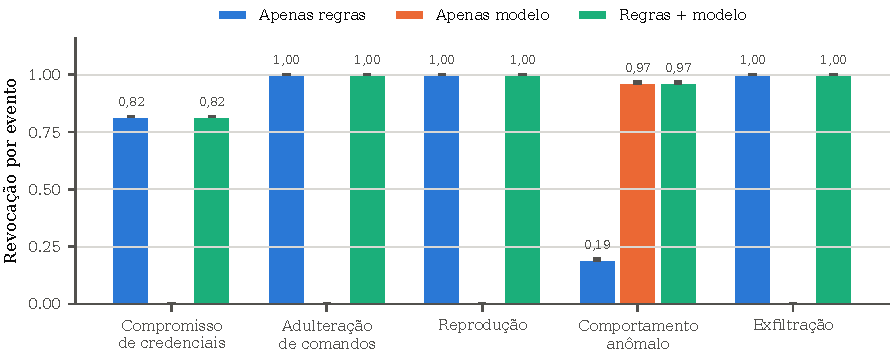
\includegraphics{figures/ablation_pt.pdf}
\caption{Revocação por evento, por cenário e configuração, média sobre
\expNumSeeds{} execuções com barras de desvio padrão. Barras ausentes são zero.
O catálogo de regras e a linha de base aprendida são complementares, não
redundantes: nenhuma configuração isolada cobre o corpus.}
\label{fig:ablation}
\end{figure*}

A ablação mostra que as duas metades são complementares e não se sobrepõem. O
modelo sozinho não detecta nada fora do plano de telemetria --- ele não tem nada
a dizer sobre uma etiqueta de autenticação forjada --- e as regras sozinhas
alcançam apenas \expRecAnomalyRules{} de revocação na deriva comportamental.
Juntos, cobrem o corpus. A configuração de modelo atinge precisão de
\expPrecisionMl{} com zero falsos positivos em qualquer execução, e isso é a
exigência de sequência da Seção~\ref{sec:model} fazendo seu trabalho: a taxa de
falsos positivos por amostra no ponto de operação é de \expFprTelemetryOp\%, mas
exceções isoladas nunca sobrevivem a três amostras consecutivas.

Os falsos positivos residuais concentram-se em duas regras e merecem ser
nomeados em vez de arredondados. A regra de viagem impossível dispara
\expFpAuthPerTrial{} vez por execução, sempre sobre o acesso \emph{legítimo} do
operador que se segue ao do atacante --- comportamento correto que uma métrica
baseada em rótulos é obrigada a contar como erro. A regra de taxa de comandos
dispara \expFpRatePerTrial{} vezes nas execuções em que dispara, sobre rajadas
nominais que cruzam um teto por operador simplesmente ajustado com aperto
excessivo. O primeiro caso é um artefato de métrica; o segundo é um defeito
genuíno de calibração.

\subsection{QP2: O que a linha de base acrescenta sobre os limites da espaçonave}

Esta é a comparação que importa operacionalmente, porque a verificação de limite
é o que uma missão já executa. A Figura~\ref{fig:leadtime} mostra a distribuição
do tempo de antecedência entre execuções: a linha de base aprendida levanta um
achado $\expLeadMean \pm \expLeadSD$~minutos antes da primeira violação de
limite (faixa de \expLeadMin--\expLeadMax~minutos, e em nenhuma execução o
limite disparou primeiro). A revocação por evento da deriva sobe de
\expRecAnomalyRules{} para \expRecAnomalousBehavior{}, e o TMD cai de
\expMttdAnomalyRules{} para \expMttdAnomalyAll{}~minutos.

\begin{figure}[t]
\centering
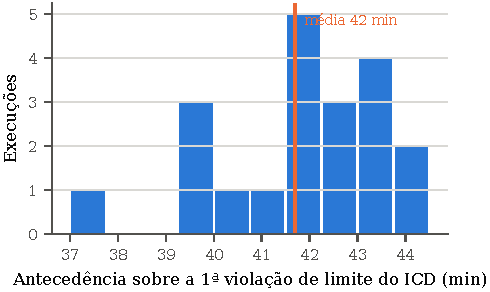
\includegraphics{figures/leadtime_pt.pdf}
\caption{Antecedência que a linha de base aprendida fornece em relação à
primeira violação de limite de controle de interface, ao longo de
\expNumSeeds{} execuções. A verificação de limite nunca disparou primeiro.}
\label{fig:leadtime}
\end{figure}

A interpretação é estreita e a enunciamos estreitamente: uma verificação de
limite informa a um operador que a espaçonave \emph{já} está fora de seu
envelope de projeto, enquanto a linha de base informa que ela está caminhando
para lá. Quarenta minutos são a diferença entre diagnosticar uma degradação e
reagir a um alarme. Isso não é evidência de que o modelo seja um bom detector de
anomalias em geral --- apenas de que é um indicador precoce melhor do que uma
linha vermelha.

\subsection{QP3: Multivariado contra univariado --- dois resultados negativos}

\emph{Na deriva injetada, a covariância não compra nada.} A
Figura~\ref{fig:roc} mostra a característica de operação do receptor de ambos os
detectores no plano de telemetria das execuções atacadas, com ampliação na única
região em que poderiam diferir. Ao longo de \expNumSeeds{} execuções, o detector
multivariado alcança $\mathrm{AUC}\ \expAucMulti \pm \expAucMultiSD$ e o melhor
canal isolado, $\expAucUni \pm \expAucUniSD$. O detector univariado é
marginalmente \emph{melhor}, e a diferença é menor do que a dispersão entre
execuções. A justificativa em torno da qual projetamos o modelo --- que a
correlação é o que torna visível um ataque sublimiar --- não se sustenta para
este ataque.

\begin{figure}[t]
\centering
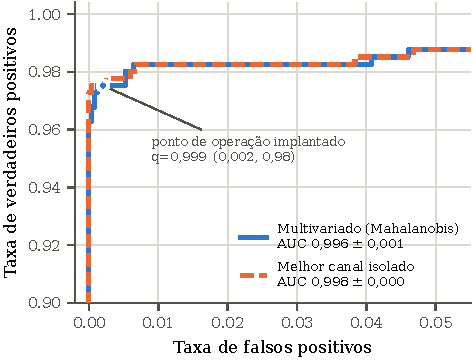
\includegraphics{figures/roc_pt.pdf}
\caption{ROC no plano de telemetria das execuções atacadas, ampliada para
$\mathrm{FPR} \le 0{,}055$; na faixa completa as duas curvas são
indistinguíveis. A AUC é a média $\pm$ desvio padrão sobre \expNumSeeds{}
execuções. O detector por canal é marginalmente melhor do que o multivariado.}
\label{fig:roc}
\end{figure}

A explicação está no ataque, não no modelo. A deriva injetada move a taxa de
manobra, a corrente do barramento e a temperatura do amplificador vários desvios
padrão robustos para fora de seus próprios centros, de modo que cada canal é
individualmente anômalo e um teste por canal basta. Uma leitura justa é que
nosso cenário comportamental é mais fácil do que se pretendia e que o
experimento não testa a alegação.

\emph{Em um ataque que isola a estrutura conjunta, ambos os detectores falham.}
A sonda de troca de fase da Seção~\ref{sec:probe} testa, sim, essa alegação, e o
resultado é pior do que inconclusivo. A Figura~\ref{fig:phaseswap} mostra por
quê: os vetores trocados não apenas deixam de exceder o limiar --- eles pontuam
\emph{abaixo} da telemetria nominal, com distância quadrática mediana de
\expSwapMedianSwapped{} contra \expSwapMedianNormal{} das amostras nominais.
Ambos os detectores ficam abaixo do acaso
($\mathrm{AUC}\ \expAucSwapMulti \pm \expAucSwapMultiSD$ multivariado,
$\expAucSwapUni \pm \expAucSwapUniSD$ univariado) e o ataque é sinalizado em
apenas \expSwapDetectedMulti{} de \expNumSeeds{} execuções.

\begin{figure}[t]
\centering
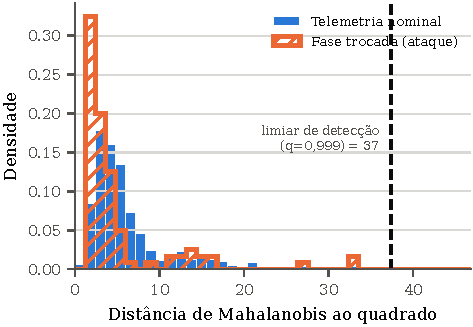
\includegraphics{figures/phaseswap_pt.pdf}
\caption{Distribuições de escore sob a sonda de troca de fase. Quadros de bordo
reproduzidos de meia órbita antes situam-se \emph{dentro} --- na verdade abaixo
--- da distribuição nominal, porque a fase orbital é marginalizada por uma linha
de base ajustada sobre uma órbita inteira. A textura é redundante com a cor,
para impressão em tons de cinza.}
\label{fig:phaseswap}
\end{figure}

Trata-se de uma limitação estrutural, não de um problema de calibração, e nenhum
limiar a resolve. Uma única gaussiana ajustada sobre uma órbita inteira aprende
a relação \emph{média} entre canais, marginalizando a fase; qualquer vetor que
tenha ocorrido em qualquer fase está, portanto, dentro da distribuição. Que as
amostras trocadas pontuem abaixo da mediana é consequência disso: valores de
meia órbita são mais densos do que os extremos que as amostras verdadeiras
ocupam. Um adversário que reproduz telemetria antiga válida se esconde dentro da
linha de base aprendida e faz a espaçonave parecer mais saudável do que está.

A correção é condicionar à fase em vez de marginalizá-la: modelar o resíduo em
relação a uma expectativa dependente da fase, ou ajustar uma mistura indexada
pela fase orbital, incluindo a fase como variável explícita de condicionamento.
Relatamos a falha em vez de implementar a correção aqui porque a sonda é a
contribuição --- é um teste barato e reutilizável ao qual qualquer detector de
telemetria de espaçonave pode ser submetido, e esperaríamos que vários
detectores publicados falhassem nele.

\subsection{QP4: De quanta telemetria limpa a linha de base precisa}

A Figura~\ref{fig:baseline} e a Tabela~\ref{tab:baseline} varrem o tamanho da
janela de treino. O achado é um limiar abrupto, não uma melhoria gradual:
ajustar com uma hora produz uma taxa de falsos positivos de telemetria de
\expFprOneHour\%, que só cai a \expFprFullDay\% quando a janela alcança
\expSimHours{} horas completas. A AUC melhora marginalmente ao longo da
varredura (\expAucBaselineMin{} a \expAucBaselineMax{}) e a taxa de verdadeiros
positivos declina levemente conforme o limiar sobe, de modo que nenhuma das duas
explica o colapso.

\begin{figure}[t]
\centering
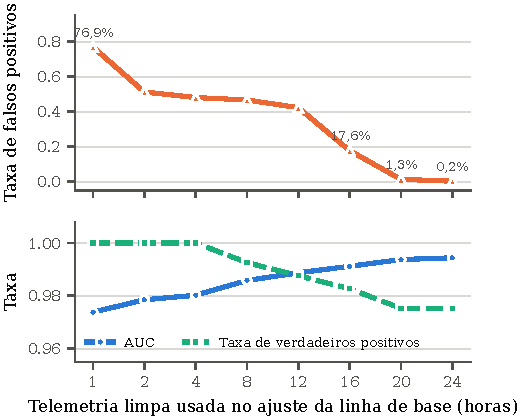
\includegraphics{figures/baseline_pt.pdf}
\caption{Sensibilidade ao tamanho da linha de base. Painel superior: taxa de
falsos positivos da telemetria no ponto de operação implantado. Painel
inferior: AUC e taxa de verdadeiros positivos. A taxa de falsos positivos só
desaba quando a janela de treino cobre um ciclo diurno completo; a discriminação
quase não muda.}
\label{fig:baseline}
\end{figure}

% Generated by paper/experiments.py -- do not edit by hand.
\begin{table}[t]
\caption{Sensibilidade ao tamanho da linha de base no ponto de operação implantado ($q = 0{,}999$). A discriminação (AUC) quase não muda; a taxa de falsos positivos só desaba quando a janela de treino cobre um ciclo diurno completo.}
\label{tab:baseline}
\centering
\begin{tabular}{@{}rrrrrr@{}}
\toprule
\textbf{Horas} & \textbf{Amostras} & \textbf{$\tau$} & \textbf{AUC} & \textbf{TPR} & \textbf{FPR (\%)} \\
\midrule
1 & 120 & 24,6 & 0,9738 & 1,000 & 76,9 \\
2 & 240 & 24,5 & 0,9785 & 1,000 & 51,2 \\
4 & 480 & 29,8 & 0,9802 & 1,000 & 48,0 \\
8 & 960 & 32,9 & 0,9858 & 0,993 & 46,6 \\
12 & 1440 & 33,5 & 0,9887 & 0,988 & 42,2 \\
16 & 1920 & 34,1 & 0,9912 & 0,983 & 17,6 \\
20 & 2400 & 34,8 & 0,9937 & 0,975 & 1,3 \\
24 & 2880 & 37,4 & 0,9944 & 0,975 & 0,2 \\
\bottomrule
\end{tabular}
\end{table}


A causa é cobertura, não tamanho de amostra. Uma janela mais curta do que o
ciclo orbital e diurno observa apenas parte do espaço de estados --- algumas
frações de eclipse, algumas geometrias de contato, alguns regimes térmicos ---
de modo que o limiar quantílico é calibrado contra uma distribuição que o modelo
implantado não verá. A regra operacional implicada é concreta: uma linha de base
deve cobrir ao menos um ciclo completo de cada periodicidade que a missão tenha,
e um detector que relatasse apenas AUC teria concluído, erradamente, que uma
hora de dados é quase tão boa quanto um dia.

\subsection{QP5: Custo}

% Generated by paper/experiments.py -- do not edit by hand.
\begin{table}[t]
\caption{Custo de detecção em um núcleo, melhor de 5 execuções sobre um corpus de 24~horas com 3584 eventos.}
\label{tab:cost}
\centering
\begin{tabular}{@{}lrr@{}}
\toprule
\textbf{Configuração} & \textbf{Eventos/s} & \textbf{$\mu$s/evento} \\
\midrule
Apenas regras & 237\,025 & 4,2 \\
Regras $+$ modelo & 103\,205 & 9,7 \\
\midrule
\multicolumn{3}{@{}l}{Ajuste da linha de base: 0,012\,s, 2880 amostras} \\
\multicolumn{3}{@{}l}{Modelo serializado: 1,5\,KB} \\
\bottomrule
\end{tabular}
\end{table}


A Tabela~\ref{tab:cost} dá o custo em um único núcleo. O motor processa
\expThroughputMl{} eventos por segundo com o modelo ativado
(\expUsPerEventMl~$\mu$s por evento) e \expThroughputRules{} sem ele; ajustar a
linha de base com um dia de telemetria leva \expFitSeconds{}~s e produz um
modelo de \expModelKb~KB. A uma cadência de telemetria de 30 segundos, um núcleo
é cerca de cinco ordens de magnitude mais rápido do que uma estação exige, de
modo que o custo de detecção não é a restrição --- transporte e armazenamento
são.

\subsection{Volume de alertas}

\begin{figure*}[t]
\centering
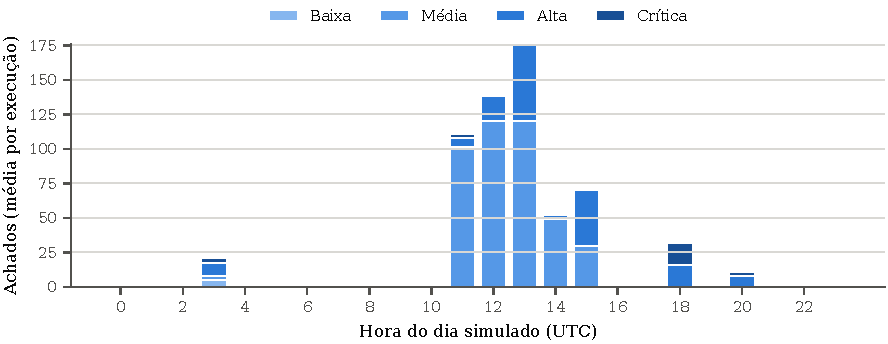
\includegraphics{figures/alerts_pt.pdf}
\caption{Achados por hora do dia simulado, por severidade, média sobre
\expNumSeeds{} execuções. A carga é em rajadas, não constante: a média diária de
\expFindingsMean{} achados não descreve nenhuma hora do dia.}
\label{fig:alerts}
\end{figure*}

A Figura~\ref{fig:alerts} mostra a carga voltada ao analista. A média de
\expFindingsMean{} achados por dia simulado é um resumo enganoso: a carga é
extremamente em rajadas, com nada por vinte horas e um pico de cerca de
\expAlertPeakHour{} achados em uma única hora, dos quais \expCriticalPerDay{}
por dia são críticos. Taxas agregadas de falsos positivos dizem pouco sobre se
uma fila é operável, e a falácia da taxa-base~\cite{axelsson2000baserate} se
aplica com toda a força nesses volumes. A mitigação prática em nosso projeto é
disciplina de severidade mais correlação: achados críticos acionam o plantão, e
as cadeias da Tabela~\ref{tab:paths} fazem com que um operador veja um incidente
em vez de quatro alertas desconexos.

\section{Discussão}

\subsection{Regras e modelos fazem trabalhos diferentes}

A ablação evidencia um ponto fácil de perder em uma área entusiasmada com
detecção aprendida: os quatro cenários de maior impacto --- comandos forjados,
reprodução, escalonamento de privilégio, exfiltração --- são capturados por
regras determinísticas, imediatamente, sem variância e sem dados de treino. São
capturados porque a missão tem uma política explícita (uma etiqueta de
autenticação deve verificar; um contador não deve repetir; um papel não pode
emitir este \emph{opcode}) e uma regra é a expressão natural de uma política. A
detecção aprendida só se paga onde não existe política a enunciar: comportamento
que é legal a cada instante e errado no agregado. Tratar detecção de anomalias
como substituto da codificação de políticas, em vez de complemento, teria
produzido um sistema que perde tudo nos três primeiros grupos da
Figura~\ref{fig:ablation}.

\subsection{O que os resultados negativos significam na prática}

Nossos dois resultados negativos apontam na mesma direção: as distribuições
marginais dos canais de bordo de uma espaçonave carregam a maior parte do sinal
que uma linha de base estática consegue extrair, e a estrutura conjunta que uma
linha de base estática aprende é grosseira demais para capturar um adversário
que respeite as marginais. Como a segunda falha fica abaixo do acaso, ela
também é \emph{explorável}: um adversário que saiba que uma linha de base do
tipo Mahalanobis está implantada pode reproduzir quadros antigos não apenas para
evadi-la, mas para empurrar o escore de anomalia para baixo enquanto uma falha
progride.

Acreditamos que a implicação generaliza além do nosso modelo. Qualquer detector
que ajuste uma distribuição marginal em fase sobre um sistema periódico herda o
mesmo ponto cego, incluindo detectores consideravelmente mais sofisticados que o
nosso~\cite{hundman2018lstm,yairi2017datadriven}, a menos que condicionem
explicitamente à fase. A sonda de troca de fase custa poucas linhas para
implementar e encorajaríamos seu uso como verificação padrão.

\subsection{Lições de implantação}

As três falhas silenciosas da Seção~\ref{sec:impl} têm a mesma forma: a API de
nuvem aceitou a requisição, devolveu sucesso e descartou os dados ou a intenção
de configuração. Uma pipeline de detecção é exatamente o tipo de sistema em que
tais falhas são invisíveis --- um grupo de \emph{logs} vazio e uma fila silenciosa
parecem idênticos a um dia tranquilo. Tiramos duas lições. Falhar ruidosamente
na aceitação parcial, mesmo quando a API não a considera erro. E testar o
caminho de nuvem, não apenas a lógica: uma emulação em processo dos serviços de
nuvem capturou os três defeitos em uma tarde, sem credenciais e sem conta.

\section{Limitações e Ameaças à Validade}
\label{sec:limitations}

\emph{O corpus é sintético.} Esta é a ameaça dominante e não a minimizamos.
Nosso modelo de espaçonave é um perfil senoidal de iluminação com atrasos
térmicos de primeira ordem; telemetria de bordo real tem não linearidade de
instrumento, falhas de sensor, deriva sazonal do ângulo beta e idiossincrasia de
operador que não reproduzimos. Números absolutos devem, portanto, ser lidos como
propriedades deste corpus, não de uma missão. Os achados comparativos e
estruturais --- a complementaridade entre regras e modelo, a ordenação dos
tempos de antecedência, a cegueira à troca de fase, o limiar de cobertura ---
dependem da \emph{estrutura} dos dados e não de sua fidelidade, e esperamos que
se transfiram; a cifra de precisão, não.

\emph{Os ataques são injetados, não executados.} Nenhum \emph{exploit} executa
contra infraestrutura real. O adversário também não é adaptativo: não observa o
detector e se ajusta, que é o pressuposto mais frágil em qualquer avaliação
estática desse tipo~\cite{sommer2010closedworld}. A sonda de troca de fase é
nossa única concessão a um adversário adaptativo --- e ela teve êxito.

\emph{A granularidade dos rótulos distorce as métricas.} A revocação é por
evento, de modo que um cenário que rotula 404 eventos e outro que rotula 7 não
são comparáveis, e o falso positivo de viagem impossível discutido na
Seção~\ref{sec:results} é comportamento correto do detector pontuado como erro.
Relatamos números por cenário para manter isso visível, em vez de resolvê-lo.

\emph{Escopo.} Uma estação, uma espaçonave, uma região. Correlação entre
estações --- o mesmo endereço de origem tocando duas estações --- é um sinal
mais forte do que qualquer estação isolada, e não a avaliamos. O estado por
contêiner no detector implantado (janelas de taxa, sequências de anomalia) é
aderente ao \emph{shard} em vez de garantido; apenas a memória de reprodução é
tornada globalmente consistente.

\emph{A avaliação de nuvem é emulada.} Os testes de integração executam contra
uma emulação em processo das APIs da AWS. Ela é fiel quanto aos comportamentos
dos quais dependemos, mas não é a AWS: não revela erros de política de
autorização, cotas de serviço nem consistência eventual. O código de
infraestrutura tem formatação verificada e foi revisado, mas não foi aplicado
contra uma conta real, e o custo e a latência da pipeline implantada são,
portanto, não medidos --- apenas o custo computacional do motor na
Tabela~\ref{tab:cost} o é.

\emph{Escopo do modelo.} Avaliamos uma única família de linha de base.
\emph{Isolation Forests}~\cite{liu2008isolation}, modelos de
sequência~\cite{hundman2018lstm} e a abordagem de agrupamento probabilístico
de~\cite{yairi2017datadriven} são as comparações óbvias e ficam para trabalho
futuro; o modelo está atrás de uma interface de escore-e-limiar justamente para
que possam ser substituídos e pontuados sobre os mesmos rótulos.

\section{Trabalhos Relacionados}

\emph{Segurança de sistemas espaciais.} Pavur e Martinovic fizeram um
levantamento da área e argumentaram que seu problema central é a ausência de
artefatos reproduzíveis e de ambientes de teste
compartilhados~\cite{pavur2020sok}; este artigo é uma resposta a esse argumento
para uma parte do sistema. Pavur et al.\ demonstraram interceptação prática de
enlaces VSAT operacionais~\cite{pavur2020vsat}, e Willbold et al.\ analisaram
\emph{firmware} real de satélites e encontraram ausência sistemática de
autenticação no caminho de comando~\cite{willbold2023space}.
Falco~\cite{falco2019principles} e Manulis et al.~\cite{manulis2021newspace}
estabelecem princípios de segurança para sistemas espaciais e para o segmento
comercial de "New Space", respectivamente. O SPARTA fornece a taxonomia de
adversários específica do espaço para a qual mapeamos~\cite{sparta}, e o
ATT\&CK, a contraparte corporativa~\cite{attack}. Nosso foco difere de todos
esses por ser a pegada em nuvem do segmento terrestre e por ser avaliado contra
rótulos em vez de argumentado.

\emph{Detecção de anomalias em telemetria de espaçonaves.} Detectar falhas em
telemetria de bordo é um campo maduro. Hundman et al.\ aplicaram LSTMs com
limiarização dinâmica não paramétrica a canais de espaçonaves da
NASA~\cite{hundman2018lstm}; Yairi et al.\ combinaram agrupamento probabilístico
com redução de dimensionalidade para dados de bordo de
satélites~\cite{yairi2017datadriven}; Chandola et al.\ fazem um levantamento da
área mais ampla~\cite{chandola2009survey}. Essa literatura visa \emph{falhas} e
suas avaliações assumem que as anomalias não são escolhidas adversarialmente.
Nosso resultado de troca de fase sugere que esse pressuposto é estrutural: uma
falha não respeitará as marginais, e um adversário respeitará.

\emph{Metodologia de avaliação de detecção.} A crítica de Sommer e Paxson ao
aprendizado de máquina para detecção de intrusão~\cite{sommer2010closedworld} e
a análise de taxa-base de Axelsson~\cite{axelsson2000baserate} moldam como
relatamos resultados --- por cenário em vez de agregados, falsos positivos sobre
eventos benignos e volume de alertas como resultado de primeira classe. Ring et
al.\ fazem um levantamento dos conjuntos de dados de IDS de
rede~\cite{ring2019datasets} cuja ausência neste domínio motivou o corpus. A
emulação automatizada de adversários no estilo do
CALDERA~\cite{applebaum2016caldera} informou o projeto de injetores
componíveis.

\emph{Normas.} O modelo de comando segue o protocolo de enlace de dados espacial
TC do CCSDS~\cite{ccsds232} e sua camada de segurança~\cite{ccsds355}; nossa
etiqueta com chave e o contador de sequência substituem os serviços de
autenticação e antirreprodução daquela camada. Os achados são emitidos em
ASFF~\cite{asff}, e a implantação tem como alvo o serviço gerenciado de estação
terrestre documentado em~\cite{awsgroundstation}.

\section{Conclusão}

Construímos um ambiente de teste aberto e rotulado para detectar ataques a
estações terrestres de satélite, e uma pipeline nativa em nuvem que detecta
cinco cenários emulados em cada uma das \expNumSeeds{} execuções, com precisão de
$\expPrecision \pm \expPrecisionSD$. O resultado que consideramos mais útil não é
esse número. É que regras determinísticas de política, e não detecção aprendida,
carregam os cenários de maior impacto; que a linha de base aprendida se paga em
exatamente um dos cinco, onde compra $\expLeadMean$~minutos sobre os próprios
limites da espaçonave; que sua maquinaria multivariada não supera um detector
por canal bem calibrado naquele cenário; e que ambos são cegos --- abaixo do
acaso --- a um adversário que reproduza telemetria válida de outra fase orbital.
O último achado é estrutural, aplica-se a qualquer linha de base marginal em
fase e é testável em poucas linhas de código.

O artefato é público, determinístico e executa \emph{offline} em segundos, de
modo que cada uma dessas afirmações pode ser verificada e, esperamos,
melhorada.

\section*{Disponibilidade}

O simulador, os cenários de ataque, o motor de detecção, o código de
infraestrutura, o arcabouço experimental e as fontes deste manuscrito estão
disponíveis em
\url{https://github.com/rikosoo/Cloud-Native-Detection-of-\allowbreak Cyberattacks-Against-Satellite-Ground-Stations}.
Executar \texttt{python paper/experiments.py} regenera todos os números e
figuras deste artigo.

\section*{Considerações Éticas}

Nenhuma estação terrestre, espaçonave ou sistema de terceiros real foi tocado.
Toda a telemetria, credenciais e registros de auditoria são sintéticos; as
chaves criptográficas no repositório são constantes de laboratório, rotuladas
como tais e inadequadas a qualquer uso operacional. Os cenários de ataque
descrevem comportamento de adversário no nível da engenharia de detecção e não
contêm código de \emph{exploit}, nenhuma vulnerabilidade em produto real e nada
que abrevie o caminho para atacar uma missão operacional.

\bibliographystyle{IEEEtran}
\bibliography{refs}

\end{document}
